\documentclass{article}
\usepackage[T1]{fontenc}
\usepackage{amsmath,amsthm}
\usepackage{amssymb}
\usepackage{color}
\usepackage{tikz}
\usetikzlibrary{shadings}
\usetikzlibrary{shapes}
\usetikzlibrary{arrows, positioning}
\tikzset{>=latex}

\begin{document}

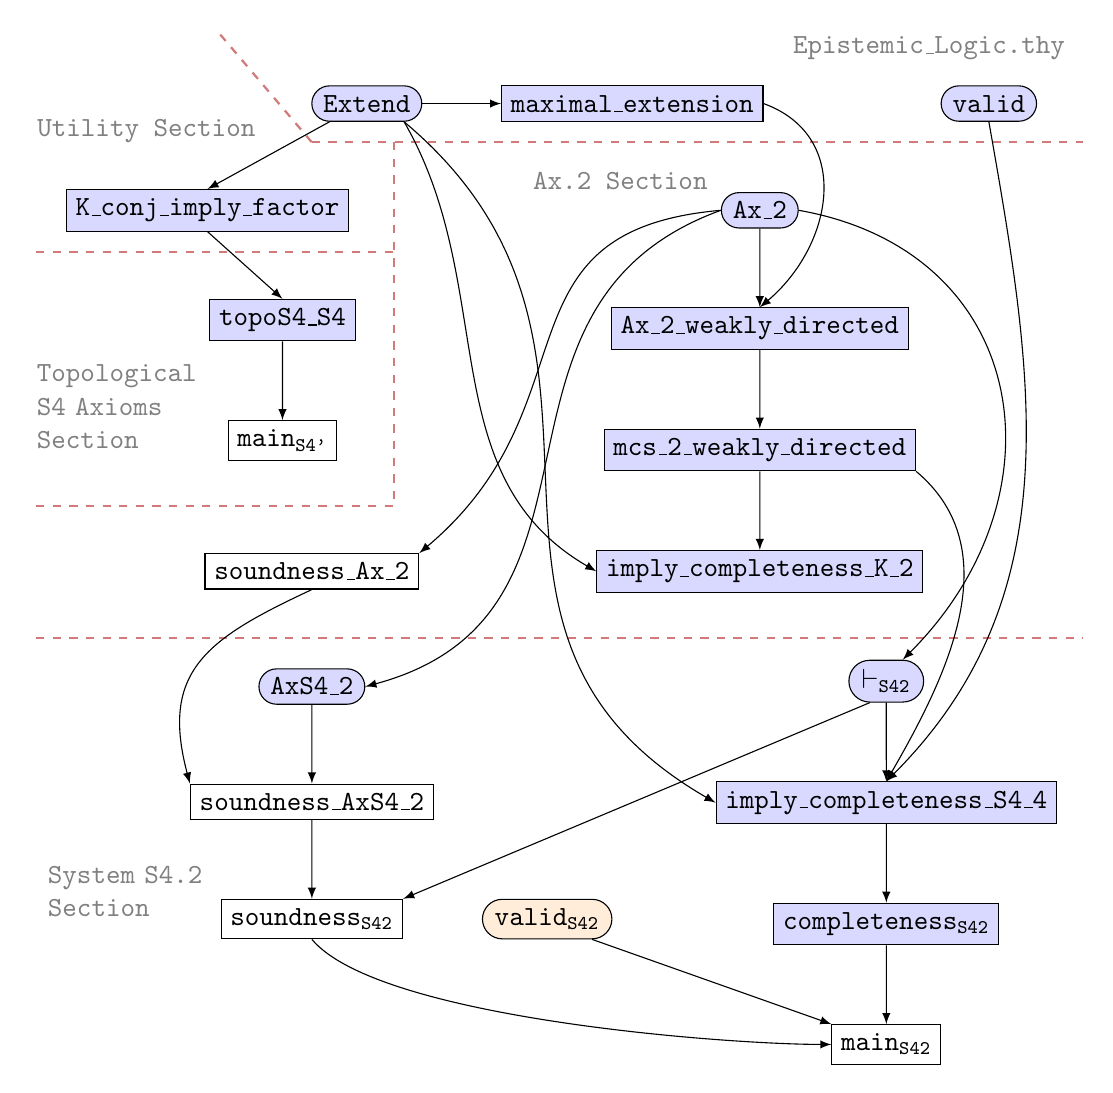
\begin{tikzpicture}[ scale=.7,
ne1/.style={rectangle, draw=black, fill=blue!15},
ne2/.style={rectangle, draw=black, fill=orange!25},
ne3/.style={rectangle, draw=black, fill=white},
de1/.style={rounded rectangle, draw=black, fill=blue!15},
de2/.style={rounded rectangle, draw=black, fill=orange!15},
de3/.style={rounded rectangle, draw=black, fill=white} ]
  \node[de1] (e1) {\texttt{Extend}};
  \node[] (y2) [below=of e1] {};
  \node[ne1] (e2) [right=of e1] {\texttt{maximal\_extension}};
  \node[] (x3) [right=of e2] {};
  \node[] (y1) [below=of e2] {};
  \node[de1] (e3) [right=of x3] {\texttt{valid}};
  \node[] (x6) [below=of e3] {};
  \draw[dashed, red!50!gray, thick, opacity=.7] (-1,-.7) -- (13,-.7);
  \draw[dashed, red!50!gray, thick, opacity=.7] (-1,-.7) -- (-2.7,1.3);
  \node[gray] (el) at (10.2,1) {\tt Epistemic\_Logic.thy};
  % ax2
  \node[de1] (a1) [right=of y1] {\texttt{Ax\_2}};
  \node[] (x2) [left=of a1] {};
  \node[ne1] (a2) [below=of a1] {\texttt{Ax\_2\_weakly\_directed}};
  \node[ne1] (a3) [below=of a2] {\texttt{mcs\_2\_weakly\_directed}};
  \node[] (x1) [left=of a2] {};
  \node[ne1] (a4) [below=of a3] {\texttt{imply\_completeness\_K\_2}};
  \node[] (x4) [left=of a4] {};
  \node[ne3] (a5) [left=of x4] {\texttt{soundness\_Ax\_2}};
  \draw[dashed, red!50!gray, thick, opacity=.7] (-6,-9.7) -- (13,-9.7);
  \node[gray] (al) at (4.6,-1.4) {\tt Ax.2 Section};
  % utility
  \node[ne1] (u1) [left=.1cm of y2] {\texttt{K\_conj\_imply\_factor}};
  \node[] (y2) [below=of u1] {};
  \draw[dashed, red!50!gray, thick, opacity=.7] (-6,-2.7) -- (0.5,-2.7);
  \node[gray] (el) at (-4,-.5) {\tt Utility Section};
  % topological
  \node[ne1] (t1) [right=-.1cm of y2] {\texttt{topoS4\_S4}};
  \node[ne3] (t2) [below=of t1] {\texttt{main$_{\texttt{S4'}}$}};
  \draw[dashed, red!50!gray, thick, opacity=.7] (-6,-7.3) -- (0.5,-7.3);
  \draw[dashed, red!50!gray, thick, opacity=.7] (0.5,-.7) -- (0.5,-7.3);
  \node[gray] (el) [text width=2.5cm] at (-4.2,-5.5) {\tt Topological S4 Axioms Section};
  % system S4.2
  \node[] (x5) [below=of a4] {};
  \node[de1] (s1) [right=of x5] {$\vdash_{\texttt{S42}}$};
  \node[] (x7) [below=of s1] {};
  \node[de1] (s2) [below=of a5] {\tt AxS4\_2};
  \node[ne3] (s3) [below=of s2] {\tt soundness\_AxS4\_2};
  \node[ne3] (s4) [below=of s3] {\tt soundness$_{\texttt{S42}}$};
  \node[ne1] (s5) [below=of s1] {\tt imply\_completeness\_S4\_4};
  \node[ne1] (s6) [below=of s5] {\tt completeness$_{\texttt{S42}}$};
  \node[de2] (s7) [right=of s4] {\tt valid$_{\texttt{S42}}$};
  \node[ne3] (s8) [below=of s6] {\tt main$_{\texttt{S42}}$};
  \node[gray] (sl) [text width=2.5cm] at (-4,-14.3) {\tt System S4.2 Section};
  % arrows
  \draw[->] (e1.south west) -- (u1.north);
  \draw[->] (e1.east) -- (e2.west);
  \draw[->] (e1.south east) to[out=300, in=150, looseness=1] (a4.west);
  \draw[->] (u1.south) -- (t1.north);
  \draw[->] (t1.south) -- (t2.north);
  \draw[->] (e2.east) to[out=340, in=40, looseness=1.2] (a2.north);
  \draw[->] (a1.south) -- (a2.north);
  \draw[->] (a1.west) to[out=185, in=40, looseness=1.3] (a5.north east);
  \draw[->] (a1.east) to[out=350, in=45, looseness=1.3] (s1.north east);
  \draw[->] (a1.west) to[out=200, in=15, looseness=1.2] (s2.east);
  \draw[->] (a2.south) -- (a3.north);
  \draw[->] (a3.south) -- (a4.north);
  \draw[->] (a5.south) to[out=205, in=105, looseness=1.3] (s3.north west);
  \draw[->] (s2.south) -- (s3.north);
  \draw[->] (s3.south) -- (s4.north);
  \draw[->] (s1.south west) -- (s4.north east);
  \draw[->] (s1.south) -- (s5.north);
  \draw[->] (e1.south east) to[out=320, in=150, looseness=1.2] (s5.west);
  \draw[->] (a3.south east) to[out=320, in=60] (s5.north);
  \draw[->] (e3.south) to[out=280, in=45, looseness=1] (s5.north);
  \draw[->] (s5.south) -- (s6.north);
  \draw[->] (s7.south east) -- (s8.north west);
  \draw[->] (s4.south) to[out=310, in=180, looseness=0.5] (s8.west);
  \draw[->] (s6.south) -- (s8.north);
\end{tikzpicture}

\end{document}